\documentclass[12pt]{article}
\usepackage[margin=2cm]{geometry}
\usepackage{cite}
\usepackage{float}
\usepackage{graphicx}
\usepackage[caption=false]{subfig}
  \DeclareGraphicsExtensions{.png}
\usepackage{amsmath}
\usepackage{amsfonts}
\usepackage{url}
\usepackage{tikz}
\usetikzlibrary{shapes,shapes.gates.logic.US,arrows,chains,calc}
\tikzset{
  -|-/.style={
    to path={
      (\tikztostart) -| ($(\tikztostart)!#1!(\tikztotarget)$) |- (\tikztotarget)
      \tikztonodes
    }
  },
  -|-/.default=0.5,
  |-|/.style={
    to path={
      (\tikztostart) |- ($(\tikztostart)!#1!(\tikztotarget)$) -| (\tikztotarget)
      \tikztonodes
    }
  },
  |-|/.default=0.5,
}
\usepackage{tikz-timing}
\usetikztiminglibrary[new={char=Q,reset char=R}]{counters}
\usepackage{bm,times}
\usepackage{pgfgantt}
\usepackage{indentfirst}
\usepackage{array}

\begin{document}
\begin{titlepage}
  { \Large
    Imperial College London\\[17pt]
    Department of Electrical and Electronic Engineering\\[17pt]
    Final Year Project Report (DRAFT)
  }

  \rule{\columnwidth}{3pt}
  \vfill
  \centering
  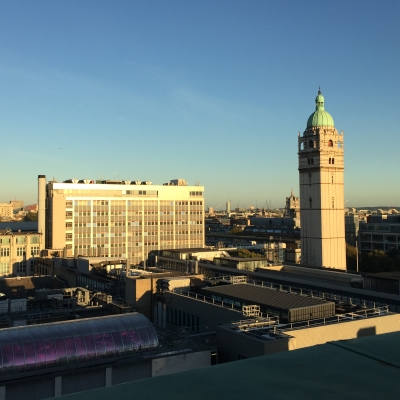
\includegraphics[width=0.7\columnwidth]{img/1.jpg}
  \vfill

  \begin{table}[h]
  \def\arraystretch{1.8}
    \begin{tabular}{p{40mm}p{\dimexpr\columnwidth-40mm}}
      Project Title: & \textbf{An Extensible Framework for \newline At-speed Evaluation of Arithmetic Hardware} \\
      Student:       & \textbf{Zifan Wang} \\
      CID:           & \textbf{01077639} \\
      Course:        & \textbf{EEE4} \\
      Project Supervisor: & \textbf{Dr. James J. Davis} \\
      Second Marker: & \textbf{Dr. Christos Bouganis}
    \end{tabular}
  \end{table}
\end{titlepage}

\newpage
\vspace*{6cm}
% An Extensible Framework for At-speed Evaluation of Arithmetic Hardware

\begin{abstract}
In this project, we aim to provide a customisable evaluation framework for arithmetic hardware.
Initially, the project was conceived to perform at-speed testing of a set of newly designed high-radix online arithmetic units.
The key benefits of this exotic configuration are its high throughput and ability to fail gracefully.
As such, the testbench is designed to have a high maximum bandwidth and a method of monitoring the precision of the errors.
However, we soon realised that in general, researchers would build their own ad-hoc testbench on FPGAs when experimenting with a new operator design.
To improve the efficiency of their research and developments, we propose a flexible evaluation system for arithmetic units with this project.
The framework includes both the testing software and the hardware architecture to minimise work for the user.
Using a Cyclone V SoC development board, the system is implemented to demonstrate that it is indeed easy to setup and use, and can be modified to accommodate a variety of testing situations.
Performance-wise, the implementation is stable at 400MHz on FPGA, resulting in a $4$ orders of magnitude acceleration compared to testing by software simulation.

\end{abstract}


\newpage

\setcounter{tocdepth}{2}
\tableofcontents

\newpage

\section{Introduction}

In this project, I will explore high-radix online operators, investigating their suitability for FPGA implementation and examining the resultant tradeoffs between performance, area and power.


\chapter{Background}



\section{Project Specification}

\subsection{Project Organisation}
This project is a part of a larger project investigating the effect of using high-radix number representation with online arithmetic operators.
The overarching aim involves implementing such a system on an FPGA and quantifying its performance improvements.
This is achieved through two individual projects, vertically split from the enveloping project.
One shall design the arithmetic operator modules, while the other shall design a system from the top-level to test and evaluate these operators.
This project deals with the system-level issues.

As this project progresses in parallel with the designing of the operator modules, it is necessary to decouple the two projects so that, being individual projects, they can be evaluated individually.
The success of one project should not be restricted by the status of the other.
To this end, the goal of the system-level design is more focussed on its functionalities and robustness.
This relationship and its effect on the evaluation will be examined further in the evaluation chapter of this report.

To ensure the two products will work together once they are both complete, a common interface is agreed upon.
The interface will be done using Qsys.
The unit-level project will build different operators, which can have varying arithmetic functions and designs.
These can be packaged into individual Qsys modules, as adders, multipliers, or dividers.
Alternatively they can also be delivered as a single module taking two operands and an instruction that is one of the four basic arithmetic operations.
These will then become the DUTs of the testbench.

\subsection{Deliverables}
At the end of the project, the system should be able to perform the following:
\begin{enumerate}
  \item Connect to the arithmetic modules as its input;
  \item Generate and run tests on these modules;
  \item Vary the frequency of the FPGA;
  \item Evaluate its performance.
\end{enumerate}

\subsection{Hardware Choice}
The system itself will be built on a Cyclone V SX SoC Development Board from Intel~\cite{Intel1}.

\begin{figure}[H]
  \centering
  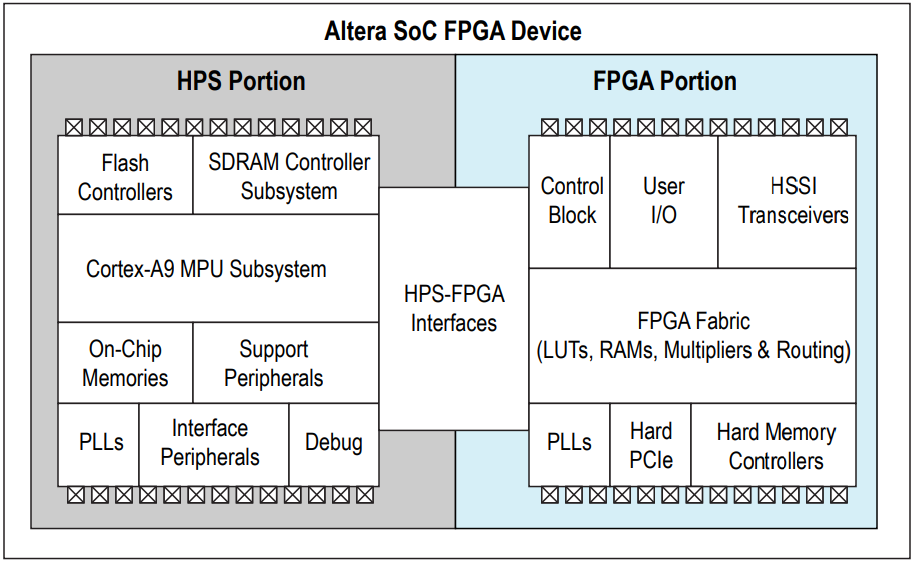
\includegraphics[width=10cm]{img/SoCStructure}
  \caption{Structure of the System-on-Chip}
  \label{SoCStructure}
\end{figure}

The 5CSXFC6D6F31C6N SoC has an Arm Cortex-A9 MPCore accompanied by Intel's 28nm FPGA fabric~\cite{Altera1}.
The FPGA is necessary for implementing the hardware design and obtaining empirical results for the project.
% maybe hybrid architecture soc makes programming it harder and it could % be used as a negative point 
While an FPGA without an embedded CPU will be enough for this project to work, having an Hard Processor System (HPS) on the same chip is useful as the test software can run on it.
The HPS is a separate piece of hardware that distinguishes itself from a soft processor, such as the Nios II, a processor programmed onto the FPGA itself.
With this additional capacity, a better user interface can thus be constructed with more detailed, on-the-fly control of the FPGA.
This means setting up the testbench will only require programming the design into the FPGA, followed by running the test script on the HPS.
The product will thus be self-contained.
It will be more accessible as no additional setup is required for the user.

It should be noted that Xilinx offers similar boards as well.
Its Zynq SoC family has a very comparable structure as they too integrate the software programmability of an Arm processor with the hardware possibility of an FPGA.
For example, similar to the Cyclone V SX, Zynq-7000S features an Arm Cortex-A9
coupled with a Xilinx 28nm FPGA~\cite{Xilinx1}.
As such, a board like the ZedBoard~\cite{Xilinx2} could be just as viable for this project.

As there are very few significant functional differences between the two brands, I shall initially explore with the Intel board, simply for its availability and my familiarity with their development tools.
Due to the architectural differences between the logic elements between Xilinx and Altera FPGAs~\cite{Scekic1}, the performances on the two boards are not necessarily identical.
Once the project has progressed to a point where the system design is mature and tested, the Xilinx alternative can be explored as an extension.

\subsection{Software Choice}
The software choice follows closely with the hardware choice in this project.
To develop for Intel FPGAs, Quartus has to be used.
The version picked is arbitrary as there are not many functional differences between the versions that will be critical to the project.
As Quartus Prime 16.0 is the version installed in the computers in the department, I will use the same version simply for convenience.
This naturally means the hardware system will be built with the system integration tool that comes with Quartus -- Qsys.

The Qsys software is designed to be used for integrating different hardware modules into a system.
As such, it will be used as the interface for the two parallel projects.

While an HLS language could be used, in this design it suffers from a few problems and does not offer enough benefits to justify its use.
Usually HLS is preferred for developing complex algorithms, because compilers can optimise them into RTL much better than humans.
However, the resulting RTL would be unreadable, making directly controlling or debugging at the hardware level nearly impossible.
The interfaces require detailed control of the actual hardware and the rest of the testbench has a lot of control path work and direct manipulation on the data bits.
It is therefore not worth it to use HLS and as such, this design will be written in Verilog.

Other than the hardware design tools, there is some freedom of choice on the HPS side of the project.
The test will be built with Python, which will be running on an Ubuntu system that is installed on the HPS.
This choice is made as there are previous unrelated projects on the same development board, which means a lot of time can be saved on tedious setup works such as getting an operating system booting.

Git is used as the version control system for this project.
A list of repositories on GitHub holds all files related to this project.
Readme files on the repositories and the commit histories will serve as digital logbooks to this project.


\section{System-level Design}

\subsection{Testbench Architecture}
The design of the verification system is the major engineering challenge of this project.
% REVISIT: this sentence should be moved to intro for overall motivation of project.
While there have been many similar performance analyses done on hybrid SoCs before, each of them used their own, usually ad hoc, testbench design~\cite{Shi1}~\cite{Li1}.
As such, most testbench are not designed to be scalable or portable, serving only what they are built for.
In this project, I shall use a generic structure inspired by that of an agent in Universal Verification Methodology (UVM).

Before UVM, integrated circuit designs were verified with methodologies developed independently by stimulator vendors such as Cadence, Mentor Graphics, and Synopsys.
In an effort to unify for greater efficiency, the standards organisation of the Electronic Design Automation (EDA) industry, Accellera, established UVM with support from multiple vendors.
It provided a common structure for verification, with class libraries that made building and running a testbench a significantly smoother experience.
The agent is a container in UVM that emulates and verifies DUTs~\cite{Accellera1}.
While this project is in no position to achieve what UVM has done, I do hope that this testbench would have an easily modifiable structure that will make the process of testing similar future designs slightly simpler.

\begin{figure}[H]
  \centering
  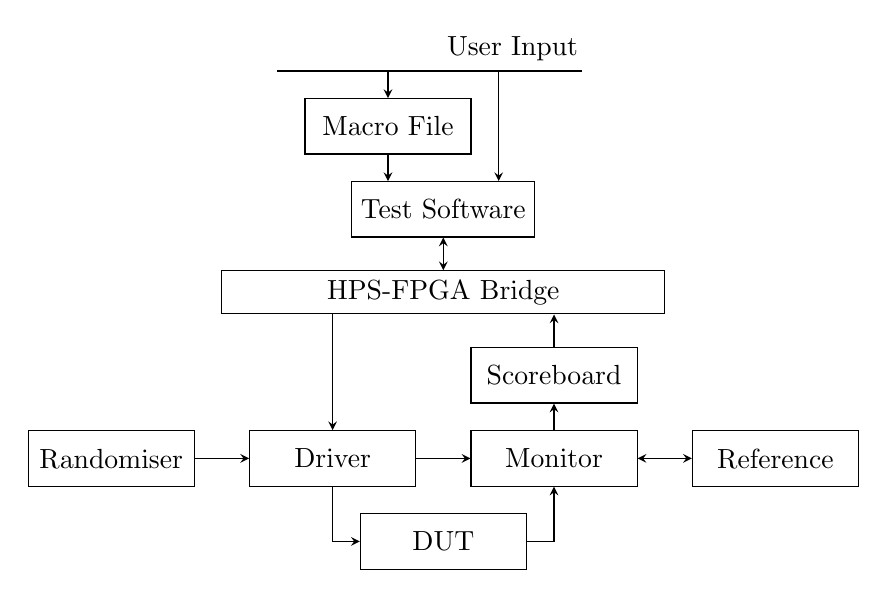
\begin{tikzpicture}
  [
    x=1em, y=1em,
    block/.style =
      {draw, rectangle, align=center, minimum width=6em, minimum height=2em},
    inter/.style =
      {draw, rectangle, align=center, minimum width=16em, minimum height=1em}
  ]
  \node [block] at (-8,3)  (r) {Randomiser};
  \node [block] at ( 0,3)  (d) {Driver};
  \node [block] at ( 4,0)  (t) {DUT};
  \node [block] at ( 8,6)  (s) {Scoreboard};
  \node [block] at ( 8,3)  (m) {Monitor};
  \node [block] at (16,3)  (u) {Reference};
  \node [inter] at ( 4,9)  (b) {HPS-FPGA Bridge};
  \node [block] at ( 4,12) (w) {Test Software};
  \node [block] at ( 2,15) (f) {Macro File};

  \draw[ ->, >=stealth] (r.east)           -- (d.west);
  \draw[ ->, >=stealth] (d.south)          |- (t.west);
  \draw[ ->, >=stealth] (t.east)           -| (m.south);
  \draw[ ->, >=stealth] (m.north)          -- (s.south);
  \draw[ ->, >=stealth] (b.south-|d.north) -- (d.north);
  \draw[ ->, >=stealth] (s.north)          -- (b.south-|s.north);
  \draw[<->, >=stealth] (b.north)          -- (w.south);
  \draw[ ->, >=stealth] (f.south)          -- (w.north-|f.north);
  \draw[ ->, >=stealth] (d.east)           -- (m.west);
  \draw[<->, >=stealth] (m.east)           -- (u.west);
  \draw[ ->, >=stealth] (2, 17)            -- (f.north);
  \draw[ ->, >=stealth] (6, 17)            -- (w.north-|6,17);

  \draw (-2,17) -- ++(6,0) -- node[above] {User Input} ++(5,0);
\end{tikzpicture}
  \caption{Block diagram of the testbench design}
  \label{Block}
\end{figure}

The test script running on the HPS will read from a configuration file, and sends the corresponding test configuration to the driver.
The driver then pulls a stream of random data generated by the randomiser, and convert them to meaningful test inputs according to specification.
The test output will be watched by the monitor, reporting any interesting event to the scoreboard, which keeps track of them.
The Monitor make uses of reference designs functionally identical to the DUT, which allows identification of false outputs from the DUT.
Multiple instances of the reference designs means multiple test data can be processed in parallel, so that the reference design can have a relaxed frequency requirement.
The scoreboard tallies the events and writes them to memory locations accessible from the other side of the bridge.
These memory locations are read by the test scripts, providing results and other useful information to the user.
The design and implementation of each individual hardware and software module will be elaborated in detail in the following chapters.

\subsection{User Interface}

For this evaluation framework to be meaningful, it has to attract users by being easy to configure and run.
To achieve this, 
% REVISIT: easy change of parameter in qsys, configuration file interface, maybe someof this is more like inplementation


\section{Hardware Design Choices}

\subsection{Data Transfer Rate}
In order to stress the DUT, the verification system must perform at a much
higher frequency than the expected frequency of the DUT.
Assuming the DUT is to run at 300MHz, to fully explore the effect of
overclocking, the testbench must be able to run at double the frequency or
higher.
This gives a target frequency of 800MHz.
Assuming a data width of 32-bit, the target data transfer rate is then 
estimated to be 25.6Gbps.

\subsubsection{\textbf{HPS-FPGA Bridge}}
As the testing is to be controlled by the HPS, the HPS-FPGA bridge will be the
immediate bottleneck if the test data is to flow from HPS to FPGA.
While the HPS can easily generate test data with a piece of software,
there is a large amount of overhead as data crosses from one architecture
to another.
This overhead exists in the form of both decreased bandwidth and increased
delay.
Thus, it is not be sensible for the HPS to send out data during runtime.

\subsubsection{\textbf{Off-chip DDR SDRAM}}
Another thought may be to first populate the off-chip DDR SDRAM on the FPGA
side, then feed that data to the DUT during test.
This is already much faster than passing the data directly from HPS.
The 1GB, 32-bit wide DDR3 on the FPGA side is rated at 400MHz.
With double rate transfer, this gives a maximum transfer rate of 25.6Gbps.

Although using the off-chip RAM may theoretically achieve the targets,
it still has its disadvantages.
Firstly, the process of filling up the memory takes time.
Thus, the testing would be broken up into bursts, with time in between for
checking results and filling in new data.
The complexity of the SDRAM interface also requires an SDRAM controller to be
used to manage SDRAM refresh cycles, address multiplexing and interface timing.
These all add up to significant access latency.
While it could be overcome with burst and piplined accesses,
it would further complicate the SDRAM controller.
A controller is provided by Intel~\cite{Altera3}, but it would consume
a non-negligible amount of the limited FPGA resources while adding
unnecessary complexities to the design.
Customising or building a new SDRAM controller to fit this project is possible,
but needlessly time-consuming.

\subsubsection{\textbf{On-chip Memory}}
The on-chip memory is much faster and simpler to use.
In comparison, this memory is implemented on the FPGA itself, and thus needs
no external connections for accesses.
It has higher throughput and lower latency than the SDRAM.
The memory transactions can also be piplined, giving one transaction per
clock cycle.
With an on-chip FIFO accessed in dual-port mode, the write operations at one
end and the read operations at the other end can happen simultaneously.
This feature is useful as tests are prepared and fed into the DUT, or when test
results are collected and fed to the monitor.

On-chip memory is not without its drawbacks.
It is volatile like SDRAM and very limited in capacity.
SDRAMs can have store about 1GB, while on-chip memory could only hold a few
MB~\cite{Altera2}.
Volatility is not exactly of concern in this project, but its small capacity
means not much test data can be held before it needs more fed in.

\subsubsection{\textbf{Distributed RAM / Registers}}
On-chip memory has a minimum latency of 1 clock cycle as the R/W access gets
processed.
If a even faster memory is desired, we can use LUTs or registers to store them.
This option would eliminate the latency but takes up much more FPGA resources.
The capacity is even more limited as LUTs are usually used for logic.
There will be a significant amount of data generated during testing, and the
testbench should be as lightweight as possible to allow flexibility in the DUTs.
As such, distributed RAM will not be used in this project for data transfer.
Registers will still be used as they are essential for many other purposes.

\subsection{Randomiser}
To exploit the benefits of on-chip memory, and circumvent the drawback of
buffering testing data generated from the HPS, a method for generating testing
data at runtime, on the FPGA needs to be designed.
As arithmetic operators have a vast set of valid inputs, it is necessary to
have cost-effective test generation.

A good choice here is to use random testing.
With relatively low effort, random testing can provide significant coverage
and discover relatively subtle errors~\cite{Duran1}.
The main drawback of random testing is the possible lack of coverage for corner
cases, for which the usual solution is to provide handwritten tests to
complement it.
However, as the main goal of this testbench is gauging the performance of
the module, and not necessarily verifying the correctness of the module,
having uncovered testing holes is acceptable during stress testing.
As the project progress, special tests could be written and run separately
with a relaxed timing restriction to cover the holes.
It should be noted that certain corner cases may represent critical paths in
the design.
To combat this, the testbench provides the option to run handwritten inputs
alongside random tests.

LFSRs are a reliable way of generating pseudorandom numbers quickly with low
cost~\cite{Hazwani1}.
They will thus form the starting point of data generation.
While it is possible for data generated to be invalid as inputs to the DUT, this
should not be the case for most benchmarks in this project.
Even if this is the case, they can be dealt later in the process by the monitor.

By following this approach, the software would only need to configure the
randomiser, and test data no longer needs to pass through the HPS-FPGA bridge.
Thus, the testbench can provide fast and constant data to stress the DUT.

\subsubsection{LFSR Configurations}

To compare, we can examine an 8-bit LFSR with taps on bit [7,5,4,3].

\textit{Fibonacci} --
Classical option, easier to write and scale in hardware.

\begin{figure}[ht]
  \centering
  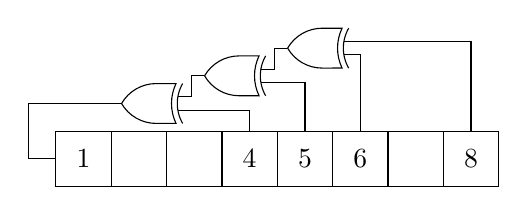
\begin{tikzpicture}
  [
    x=1em, y=1em,
    start chain = going right,
    node distance = 0em,
    reg/.style =
      {draw, minimum width=2em, minimum height=2em,outer sep=0pt, on chain},
    every join/.style={-, thick}
  ]
  \node [reg] at (0, 0) (1) {1};
  \node [reg] (2) {};
  \node [reg] (3) {};
  \node [reg] (4) {4};
  \node [reg] (5) {5};
  \node [reg] (6) {6};
  \node [reg] (7) {};
  \node [reg] (8) {8};

  \node[xor gate US,draw,rotate=180] at (2.5, 2) (a) {};
  \node[xor gate US,draw,rotate=180] at (5.5, 3) (b) {};
  \node[xor gate US,draw,rotate=180] at (8.5, 4) (c) {};

  \draw (4.north)  |- (a.input 1);
  \draw (5.north)  |- (b.input 1);
  \draw (6.north)  |- (c.input 1);

  \draw (b.output) to[-|-] (a.input 2);
  \draw (c.output) to[-|-] (b.input 2);
  \draw (8.north)       |- (c.input 2);

  \draw (a.output) -- (-2, 2) |- (1.west);

\end{tikzpicture}
  \caption{Fibonacci Configuration}
  \label{FibLFSR}
\end{figure}

\textit{Galois} --
Harder to write if variable length is desired, but faster in hardware.

\begin{figure}[ht]
  \centering
  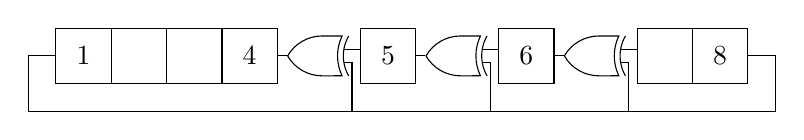
\begin{tikzpicture}
  [
    x=1em, y=1em,
    start chain = going right,
    node distance = 0em,
    reg/.style =
      {draw, minimum width=2em, minimum height=2em, outer sep=0pt, on chain},
    spa/.style =
      {minimum width=3em, minimum height=2em, outer sep=0pt, on chain},
    every join/.style={-, thick}
  ]
  \node [reg] at (0, 0) (1) {1};
  \node [reg] (2) {};
  \node [reg] (3) {};
  \node [reg] (4) {4};
  \node [spa] ()  {};
  \node [reg] (5) {5};
  \node [spa] ()  {};
  \node [reg] (6) {6};
  \node [spa] ()  {};
  \node [reg] (7) {};
  \node [reg] (8) {8};

  \node[xor gate US,draw,rotate=180] at  (8.5, 0) (a) {};
  \node[xor gate US,draw,rotate=180] at (13.5, 0) (b) {};
  \node[xor gate US,draw,rotate=180] at (18.5, 0) (c) {};

  \draw (1.west) -| (-2, -2) -- (25,-2) |- (8.east);

  \draw  (9.7,-2) |- (a.input 1);
  \draw (14.7,-2) |- (b.input 1);
  \draw (19.7,-2) |- (c.input 1);

  \draw (a.input 2-|5.west) -- (a.input 2);
  \draw (b.input 2-|6.west) -- (b.input 2);
  \draw (c.input 2-|7.west) -- (c.input 2);

  \draw (a.output) -- (4.east);
  \draw (b.output) -- (5.east);
  \draw (c.output) -- (6.east);

\end{tikzpicture}
  \caption{Galois Configuration}
  \label{GalLFSR}
\end{figure}

\textit{Others} --
Other LFSR configurations such as Xorshift~\cite{Marsaglia1} exists, but they are much slower in hardware.

\subsubsection{Randomiser Structure}

\textit{Horizontal} --
Easy to build, easy to test with.

\begin{figure}[ht]
  \centering
  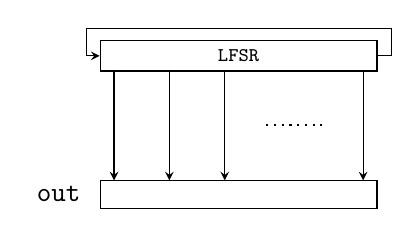
\begin{tikzpicture}
  [
    x=1em, y=1em
  ]
  \node at (-1.5, 0) {\texttt{out}};
  \node [draw,minimum height=1em, minimum width=10em] at (5, 0) (o) {};
  \node [draw,minimum height=1em, minimum width=10em] at (5, 5) (1) {\scriptsize \texttt{LFSR}};
  \draw [->, >=stealth] (1.east) -| ++(0.5, 1) -- ++(-11, 0) |- (1.west);
  \foreach \pos [count=\idx] in {0.5, 2.5, 4.5, 9.5}{
    \draw [->, >=stealth] (\pos, 4.5) -- (\pos, 0.5);
  }
  \draw [dotted, thick] (6, 2.5) -- (8, 2.5);

\end{tikzpicture}
  \caption{Horizontal Structure}
  \label{HoriLFSR}
\end{figure}

\textit{Vertical} --
Nice randomness, more scalable, need to seed all the LFSRs differently.

\begin{figure}[ht]
  \centering
  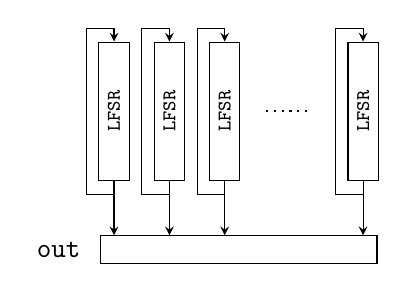
\begin{tikzpicture}
  [
    x=1em, y=1em
  ]
  \node at (-1.5, 0) {\texttt{out}};
  \node [draw,minimum height=1em, minimum width=10em] at (5, 0) (o) {};
  \foreach \pos [count=\idx] in {0.5, 2.5, 4.5, 9.5}{
    \node [draw,minimum height=1em, minimum width=5em, rotate around={90:(0, 0)}] at (\pos, 5) (\idx) {\scriptsize \texttt{LFSR}};
    \draw [->, >=stealth] (\idx.west) -- (\idx.west|-o.north);
    \draw [->, >=stealth] ($(\idx.west)-(0, 0.5)$) -| (\pos-1,8) -| (\idx.east);
  }

  \draw [dotted, thick] (6, 5) -- (7.5, 5);

\end{tikzpicture}
  \caption{Vertical Structure}
  \label{VertLFSR}
\end{figure}

\subsection{Driver}
\subsubsection{Dual Driver System}
One driver focusses on fast stress tests,
The other allows handwritten tests to coexist with random tests.
They can be switched in software.

\subsection{Monitor}

Another concern in the system design is of the different clock domains that
must exist on the FPGA.
At a minimum, there need to be two clock domains: one surrounds the DUT and
another supports the rest of the control logic around the DUT.
These clock frequencies can be generated with PLLs, which are
provided as IP Cores in the Quartus software~\cite{Altera4}.
A clock tree will distribute them to the individual modules.
Data crossing clock domains will be fed through FIFOs to prevent loss.

The proposed structure will have the bulk of the control logic running
in a separate clock domain to the DUT.
Only an interface with FIFOs will be running in synchronicity
with the DUT.
Therefore, the test controls can run at a slower frequency without
bottlenecking the system, allowing the DUT to be stressed further.
The problem now is to ensure the monitor can handle the stream of DUT output
coming in at a higher frequency that it is running at.
As the monitor needs to calculate the correct data before it can check if the
DUT output is correct, it cannot keep up with the speed of the DUT.
This report consider three alternatives.

\subsubsection{Partial Monitors}
A lightweight idea is to implement a parity checker instead of a full model
inside the monitors.
For example, to check an adder, the monitor can just check if the final bit
with a LUT acting as a XOR gate.

Although this is reasonably fast, it cannot be extended once the DUT is faster
than a parity calculation followed by a comparison.
More critically, it provides no additional information once the DUT fails, and
it has a 50\% rate of ignoring an error.
If this is to be solved by increasing the number of bits checked, the problem
returns back to its initial state.
Thus this method will not be experimented.

\subsubsection{Lazy Monitors}

\begin{figure}[H]
  \centering
  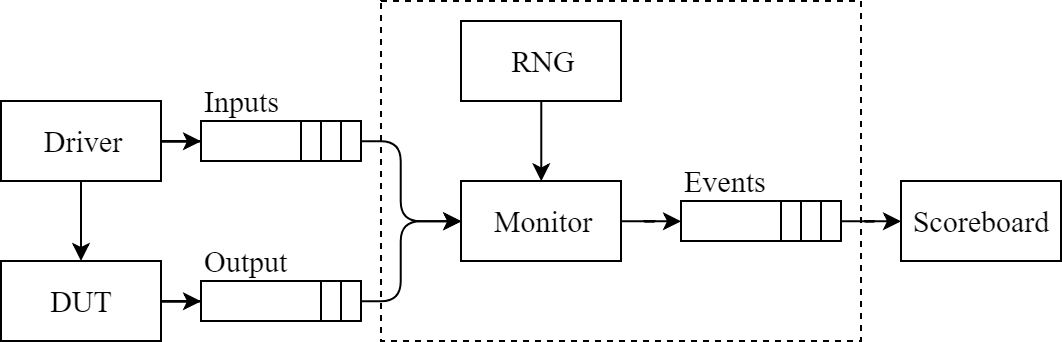
\includegraphics[width=12cm]{img/LazMon}
  \caption{Structure of a Lazy Monitor}
  \label{LazMon}
\end{figure}

An more scalable alternative is to have the monitor only check a selection of
data sets.
For example, if the monitor is programmed to check every third test point,
statistically it will make little difference to the final result.
In case the DUT is aware of this and only produce correct outputs on every third
operation, this process can be randomised too.

This method can be extended if the DUT get fast simply by skipping more checks,
and it has the full information when it detects an error.
However, this method needs the extra logic in the random controller, making the
monitor slightly more complex than it probably should be.

\subsubsection{Parallel Monitors}

\begin{figure}[H]
  \centering
  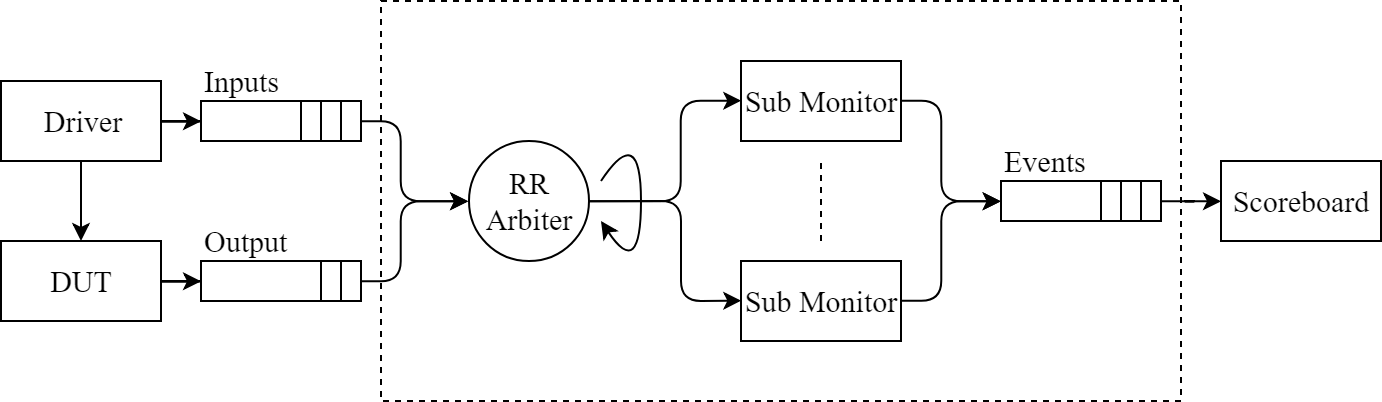
\includegraphics[width=15cm]{img/ParMon}
  \caption{Structure of a Parallel Monitor}
  \label{ParMon}
\end{figure}

As the test data is uniform, the monitor can be parallelised in to a number of
sub-monitors.
The sub-monitors is connected to a arbiter that is connected to three FIFOs.
The FIFOs are the inputs and the output of the DUT.
A round robin arbiter distributes the data to the sub-monitors equally.
The results from each sub-monitor are then sent to a single scoreboard.
To avoid potential hazards, the output from the sub-monitors will be buffered
before processed by the scoreboard.

This does not have data dependency on a random controller, and it can
fully guarantee the correctness of the DUT.
It is also scalable as more sub-monitors can be added it the DUT fills up its
output buffer.
As a downside, this method takes up the most FPGA resources to implement as it
scales.

Comparing across the three methods, the parallel monitors will be built first
for this project, as it offers the best functionalities.
Although unlikely, if a fatal issue arises in this design, or if the testbench
needs to be more lightweight, then the lazy monitor will be used as the
alternative.

\subsection{Scoreboard}

If the monitor detects an interesting event such as an error, it will send
a message to the scoreboard.
The scoreboard has counters tracking these events, which are exposed and can be
read by the HPS.

The software can run statistics to provide further insights to the user.


\section{Software Design}

\subsection{Code Structure}
The test script runs on the HPS of SoC board, providing an interface for the user to run their tests on the FPGA.
It is able to control the frequency of the FPGA and configure the testbench according to the need of the user.
It should also read from the scoreboard to results to the user.

\subsection{Software Configuration}
In order to improve usability, the user interface of the software should not include direct manipulation of the code.
While this is not an excuse for messy and unreadable code, having a separate configuration file is much more user friendly.
This configuration file will use a simple syntax to make all the options available to edit.
The software can then parse these and run accordingly.


\chapter{Hardware Implementation}

\section{Randomiser}

\begin{figure}[H]
  \centering
  \begin{tikzpicture}
  [
    x=1em, y=1em,
    block/.style =
      {draw, rectangle, align=center, minimum width=4em, minimum height=5em},
    sarrow/.style =
      {>={Stealth}, font=\ttfamily},
    darrow/.style =
      {double distance=1.5pt, >={Stealth}, font=\ttfamily}
  ]

\node[block, label=above:Randomiser] (r) at (0,0) {};

\draw [<-, sarrow] ($(r.west)+(0,2)$) -- ++(left:3) node[left] {clk};
\draw [<-, sarrow] ($(r.west)+(0,1)$) -- ++(left:3) node[left] {reset};

\draw [<-, sarrow] ($(r.west)-(0,1)$) -- ++(left:3) node[left] {enable};
\draw [<-, sarrow] ($(r.west)-(0,2)$) -- ++(left:3) node[left] {initial};

\draw [->, darrow] ($(r.east)-(0,2)$) -- ++(right:3) node[right] {out};

\end{tikzpicture}
  \caption{Randomiser Block Diagram}
  \label{RandomiserBlk}
\end{figure}

Implementing the randomiser is straight forward.
A possible set of taps for a 32-bit Galois LFSR is [32, 30, 26, 25].
Referring back at Figure~\ref{GalLFSR} on page~\pageref{GalLFSR},
the logic is to XOR the bits left of the taps with bit 0, and simple right shift for all other bits.
For driver to control the randomiser, an enable signal and an initial signal is added as input in addition to clock and reset.
The \texttt{initial} signal seeds the LFSR.

\section{Driver}

\begin{figure}[H]
  \centering
  \begin{tikzpicture}
  [
    x=1em, y=1em,
    block/.style =
      {draw, rectangle, align=center, minimum width=4em, minimum height=10em},
    sarrow/.style =
      {>={Stealth}, font=\ttfamily},
    darrow/.style =
      {double distance=1.5pt, >={Stealth}, font=\ttfamily}
  ]

\node[block, label=above:Driver] (r) at (0,0) {};
\node[draw, opacity=0, rectangle, minimum width=30em] () at (0,0) {};

\draw [<-, sarrow] ($(r.west)+(0,4.5)$) -- ++(left:3) node[left] {clk};
\draw [<-, sarrow] ($(r.west)+(0,3.5)$) -- ++(left:3) node[left] {reset};

\draw [<-, sarrow] ($(r.west)+(0,1.5)$) -- ++(left:3) node[left] {f\_select};
\draw [<-, darrow] ($(r.west)+(0,0.5)$) -- ++(left:3) node[left] {f\_manual};
\draw [<-, sarrow] ($(r.west)-(0,0.5)$) -- ++(left:3) node[left] {f\_bitset};
\draw [<-, sarrow] ($(r.west)-(0,1.5)$) -- ++(left:3) node[left] {f\_bitclr};
\draw [<-, darrow] ($(r.west)-(0,2.5)$) -- ++(left:3) node[left] {rand\_*};

\draw [<-, darrow] ($(r.west)-(0,4.5)$) -- ++(left:3) node[left] {dut\_out};

\draw [->, sarrow] ($(r.east)-(0,1.5)$) -- ++(right:3) node[right] {dut\_delay};

\draw [->, darrow] ($(r.east)-(0,3.5)$) -- ++(right:3) node[right] {drive\_*};
\draw [->, darrow] ($(r.east)-(0,4.5)$) -- ++(right:3) node[right] {drive\_delayed\_*};
\end{tikzpicture}
  \caption{Driver Block Diagram}
  \label{DriverBlk}
\end{figure}

The filter select signal \texttt{f\_select} selects the mode of operation of the driver.
When it is set, the driver will read from \texttt{f\_manual} and feed them to the output.
Otherwise, the driver will take the output of the randomisers at \texttt{rand\_*}, set and clearing specific bits according to \texttt{f\_bitset} and \texttt{f\_bitclr}.

The output is immediately sent to the DUT from the ports \texttt{drive\_dut\_*}.
The output is also delayed for a number of cycles before being sent to the monitor from the ports \texttt{drive\_mon\_*}.
This delay is known and thus can be configured by the user before compiling the testbench.

\begin{figure}[H]
  \centering
  \begin{tikztimingtable}
  [
    xscale=4,
    timing/d/background/.style={fill=white},
    timing/font=\ttfamily
  ]
  clk        & h 21{c} \\
  rand       & D{a4fe}D{527f}D{a93f}D{d49f}D{ea4f}D{7527}D{ba93}D{5d49}D{2ea4}D{1752}D{8ba9} \\
  f\_bitset  & 4D{0000} 7D{0004} \\
  f\_bitclr  & 3D{0000} 3D{f000} 5D{0000} \\
  drive\_dut & U D{a4fe}D{527f}D{a93f}D{049f}D{0a4f}D{0527}D{ba97}D{5d4d}D{1756}D{8bad} \\
  drive\_mon & 3U D{a4fe}D{527f}D{a93f}D{049f}D{0a4f}D{0527}D{ba97}D{5d4d} \\
  dut\_out   & 3U D{a4fe}D{527f}D{a93f}D{049f}D{0a4f}D{0527}D{ba97}D{5d4d} \\
\extracode
  % Add vertical lines in two colors
  \begin{pgfonlayer}{background}
    \begin{scope}[semitransparent,semithick]
      \vertlines{1,2,...,10}
    \end{scope}
  \end{pgfonlayer}
\end{tikztimingtable}
  \caption{Driver Waveform}
  \label{DriveWave}
\end{figure}

Figure \ref{DriveWave} shows how the waveform of the implemented driver looks like when operating in auto mode.
It should be stated that all waveforms in this report has been obtained from simulation, and are verified to be correct.
For clarity, unnecessary signals and signal values are omitted.

In the example waveform, we assume the design is a simple 1 input 1 output module where the input is passed to the output after 2 cycles.
The driver passed \texttt{rand} to \texttt{drive\_dut} after a cycle.
When \texttt{f\_bitclr} is \texttt{0xf000}, the top 4 bits of the output are set to 0, and when \texttt{f\_bitset} is \texttt{0x0004}, bit 2 of the output is set to 1.
It should be noted, that if the same bit is set and cleared by the user, \texttt{f\_bitclr} takes priority.
This is an arbitrary choice, and is noted in the user guide.

The driver delays the output to monitor by 2 cycles, and we can see that this aligns it the output from the DUT.

\section{Monitor}
\begin{figure}[H]
  \centering
  \begin{tikzpicture}
  [
    x=1em, y=1em,
    block/.style =
      {draw, rectangle, align=center, minimum width=4em, minimum height=5em},
    sarrow/.style =
      {>={Stealth}, font=\ttfamily},
    darrow/.style =
      {double distance=1.5pt, >={Stealth}, font=\ttfamily}
  ]

\node[block, label=above:Monitor] (r) at (0,0) {};
\node[draw, opacity=0, rectangle, minimum width=30em] () at (0,0) {};

\draw [<-, sarrow] ($(r.west)+(0,2)$) -- ++(left:3) node[left] {clk};
\draw [<-, sarrow] ($(r.west)+(0,1)$) -- ++(left:3) node[left] {reset};

\draw [<-, darrow] ($(r.west)-(0,1)$) -- ++(left:3) node[left] {drive\_mon\_*};
\draw [<-, darrow] ($(r.west)-(0,2)$) -- ++(left:3) node[left] {dut\_out};

\draw [->, sarrow] ($(r.east)-(0,1)$) -- ++(right:3) node[right] {mon\_ready};
\draw [->, darrow] ($(r.east)-(0,2)$) -- ++(right:3) node[right] {diff};

\end{tikzpicture}
  \caption{Monitor Block Diagram}
  \label{MonitorBlk}
\end{figure}

The monitor takes DUT inputs from the driver, and distributes them to a few sub-monitors.
Each sub-monitor containing a reference design then produces the correct results \texttt{mon\_out} from the inputs with a relaxed time budget.
The monitor then checks the difference between the reference output, \texttt{mon\_out}, and the DUT output, \texttt{dut\_out} with XOR gates.
This results in \texttt{diff}, where each bit set to 1 indicates a wrong bit in the DUT output.
\texttt{mon\_ready} will be set after the distributor has completed an entire round, where the first meaningful \texttt{diff} value becomes available.

As the number of sub-monitors and the width of the tested unit are parametrised, the design of the distributor was not straightforward.
An one-hot counter is set up to determined the currently active sub-monitor.
Since the sub-monitors are clocked \texttt{NUM\_SUB\_MON} times slower, an array of \texttt{NUM\_SUB\_MON} registers each of size \texttt{WIDTH} is also created for each input or output of the design.
These serves as the interface between the sub-monitors and the rest of the design.

\subsection{Sub-monitors}

\begin{figure}[H]
  \centering
  \begin{tikzpicture}
  [
    x=1em, y=1em,
    block/.style =
      {draw, rectangle, align=center, minimum width=4em, minimum height=5em},
    sarrow/.style =
      {>={Stealth}, font=\ttfamily},
    darrow/.style =
      {double distance=1.5pt, >={Stealth}, font=\ttfamily}
  ]

\node[block, label=above:Sub-monitor] (r) at (0,0) {};
\node[draw, opacity=0, rectangle, minimum width=30em] () at (0,0) {};

\draw [<-, sarrow] ($(r.west)+(0,2)$) -- ++(left:3) node[left] {clk};
\draw [<-, sarrow] ($(r.west)+(0,1)$) -- ++(left:3) node[left] {reset};

\draw [<-, darrow] ($(r.west)-(0,1)$) -- ++(left:3) node[left] {i*};
\draw [<-, darrow] ($(r.west)-(0,2)$) -- ++(left:3) node[left] {dut\_out};

\draw [->, darrow] ($(r.east)-(0,1)$) -- ++(right:3) node[right] {mon\_out};
\draw [->, darrow] ($(r.east)-(0,2)$) -- ++(right:3) node[right] {dtm\_out};

\end{tikzpicture}
  \caption{Sub-monitor Block Diagram}
  \label{SubmonBlk}
\end{figure}

The current sub-monitor is a part of the monitor module in the architecture design that interfaces with the reference module.
In addition to connecting with the reference inputs and outputs, the sub-monitors also handles the delay of the reference module.
This is due to the highly parametrised nature of the monitor module, which made it rather complex and inflexible to the addition of more features.

As such, there is an extra signal of \texttt{dtm\_out}, which has the same value as \texttt{dut\_out}, but delayed by the number of cycles that the reference design needs to complete its operation, thus aligning with \texttt{mon\_out}.
The other signals are directly connected to the reference module.

\begin{figure}[H]
  \centering
  \begin{tikztimingtable}
  [
    xscale=4,
    timing/d/background/.style={fill=white},
    timing/font=\ttfamily
  ]
  clk           & h 19{c} \\
  dist\_ctr     & D{100} 3{D{001}D{010}D{100}} \\
  drive\_mon\_a & U D{0123} 2U D{3210} 2U D{0213} 2U \\
  drive\_mon\_b & U D{4567} 2U D{7654} 2U D{4657} 2U \\
  dut\_out      & U D{468a} 2U D{a861} 2U D{486a} 2U \\
  clk\_sub  [0] & 2L 2{2{c} 2L} 2{c} L \\
  a         [0] & 2U 3D{0123} 3D{3210} 2D{0213} \\
  b         [0] & 2U 3D{4567} 3D{7654} 2D{4657} \\
  dut\_o    [0] & 2U 3D{468a} 3D{a861} 2D{486a} \\
  mon\_o    [0] & 2U 3D{468a} 3D{a864} 2D{486a} \\
  diff          & 2U 3U D{0000} 2U D{0005} U \\
\extracode
  % Add vertical lines in two colors
  \begin{pgfonlayer}{background}
    \begin{scope}[semitransparent,semithick]
      \vertlines{1,2,...,9}
    \end{scope}
  \end{pgfonlayer}
\end{tikztimingtable}
  \caption{Monitor Waveform}
  \label{MonitorWave}
\end{figure}

Figure \ref{MonitorWave} shows the waveform of a monitor with \texttt{NUM\_SUB\_MON} as 3.
The reference adder takes 1 cycle to complete, but it must be clocked at a frequency slower than that of the adder DUT.
With 3 sub-monitors, the width of \texttt{dist\_ctr} is 3, and its lowest bit corresponds to sub-monitor 0, which is shown in detail in this figure.
\texttt{clk\_sub} is the clock driving the sub-monitor, which is made by masking the DUT clock with a delayed version of \texttt{dist\_ctr}.
As it ticks, the I/O values are copied into the register arrays and held for 3 cycles.
Within this time, the reference design completes its operation, fixing the value on \texttt{mon\_o}.
When the cycle of \texttt{dist\_ctr} goes a full cycle and the \texttt{sub\_clk} ticks again, this value is collected back and XOR'ed to form the final output of the monitor, \texttt{diff}.
In the example of Figure \ref{MonitorWave}, the second result was an error on the DUT, as it gave \texttt{0xa861} while the reference answer was \texttt{0xa864}.
This means bit 0 and 2 were different, and \texttt{diff} is thus \texttt{0x0005}.

The other sub-monitors all work identically but each 1 DUT cycle later the last.
This allows the reference design to run slower than the DUT, to still provide a constant stream of \texttt{diff} at the monitor output as designed.

\section{Scoreboard}

\begin{figure}[H]
  \centering
  \begin{tikzpicture}
  [
    x=1em, y=1em,
    block/.style =
      {draw, rectangle, align=center, minimum width=4em, minimum height=7em},
    sarrow/.style =
      {>={Stealth}, font=\ttfamily},
    darrow/.style =
      {double distance=1.5pt, >={Stealth}, font=\ttfamily}
  ]

\node[block, label=above:Scoreboard] (r) at (0,0) {};
\node[draw, opacity=0, rectangle, minimum width=30em] () at (0,0) {};

\draw [<-, sarrow] ($(r.west)+(0,3)$) -- ++(left:3) node[left] {clk};
\draw [<-, sarrow] ($(r.west)+(0,2)$) -- ++(left:3) node[left] {reset};

\draw [<-, sarrow] ($(r.west)+(0,0)$) -- ++(left:3) node[left] {freeze};
\draw [<-, sarrow] ($(r.west)-(0,1)$) -- ++(left:3) node[left] {mon\_ready};

\draw [<-, darrow] ($(r.west)-(0,3)$) -- ++(left:3) node[left] {diff};

\draw [->, sarrow] ($(r.east)+(0,1)$) -- ++(right:3) node[right] {maxacc};
\draw [->, sarrow] ($(r.east)+(0,0)$) -- ++(right:3) node[right] {minacc};

\draw [->, sarrow] ($(r.east)-(0,2)$) -- ++(right:3) node[right] {data\_ctr};
\draw [->, sarrow] ($(r.east)-(0,3)$) -- ++(right:3) node[right] {error\_ctr};

\end{tikzpicture}
  \caption{Scoreboard Block Diagram}
  \label{ScoreboardBlk}
\end{figure}

This scoreboard tracks the number of valid test points going through with \texttt{data\_ctr} and the number of errors within them with \texttt{error\_ctr}.
The external input \texttt{freeze} is exposed to the software to stop all counting in the scoreboard.
As the current HPS-FPGA bridge set up only allows sequential reads to the FPGA registers, it is necessary to ensure the values do not change within a single set of read commands from the software.

Another implication of the current bridge set up is that there is no simple way of getting all the \texttt{diff} values out to the HPS for statistics calculations.
This is a limitation of the current implementation, and will be discussed in the Further work section of this report.
Therefore, the hardware will have to do some simple statistics.

Since we are interested in how the precision of the DUT degrades as the frequency increases, two signals are created to record the maximum and the minimum precision of the DUT output.
Calculating the precision with the \texttt{diff} signal means counting the number of leading zeros (\texttt{CLZ}), as zeros indicate the correct bits.
As the current implementation is limited with a maximum width of 32, the easiest way of doing \texttt{CLZ} fast is by padding zeros after the number to 32 bits, and then use a large lookup table with don't cares.
This precision signal is named \texttt{acc}.

To keep track of the minimum precision, register \texttt{minacc} is first initialised to the maximum, and then for each smaller value observed, it will take on its smaller value.
The comparison logic here is relatively expensive in this fast testbench design.
As such, there is great incentive in the future to build a better communication method to allow offloading these operations to the HPS.

\begin{figure}[H]
  \centering
  \begin{tikztimingtable}
  [
    xscale=4,
    timing/d/background/.style={fill=white},
    timing/font=\ttfamily
  ]
  clk        & h 19{c} \\
  freeze     & 8L 2H \\
  mon\_ready & 2L 8H \\
  diff       & D{000f}D{0001}D{0000}D{0001}D{000c}2D{0000}3D{0001} \\
  data\_ctr  & 3D{0} 1R 6{Q} D{0} \\
  error\_ctr & 4D{0} D{1} 3D{2} D{3} D{4} \\
  maxacc     & 3D{0} 7D{16} \\
  minacc     & 3D{16} D{15} 6D{12} \\
\extracode
  % Add vertical lines in two colors
  \begin{pgfonlayer}{background}
    \begin{scope}[semitransparent,semithick]
      \vertlines{1,2,...,9}
    \end{scope}
  \end{pgfonlayer}
\end{tikztimingtable}
  \caption{Scoreboard Waveform}
  \label{ScoreboardWave}
\end{figure}

Figure \ref{ScoreboardWave} shows a example waveform.
The counters and the extrema trackers changes value only if we have \texttt{mon\_ready \&\& !freeze}.

\section{Wrappers}

Figure \ref{DBlock} provides a detailed look at how the individual hardware components are wired together to form the \texttt{testbench} module.
The DUT is shown as internal for clarity and it is the case during simulation testing of the testbench, but it should be understood that the DUT module is external in actual use.
The reference module similarly, is implied to be contained within the sub-monitor module, but this can be external during hardware use.

\begin{figure}[H]
  \centering
  \begin{tikzpicture}
  [
    x=1em, y=1em,
    block/.style =
      {draw, rectangle, align=center, minimum width=4em, minimum height=11em},
    sarrow/.style =
      {>={Stealth}, font=\ttfamily},
    darrow/.style =
      {double distance=1.5pt, >={Stealth}, font=\ttfamily}
  ]

\node[block, label=above:Wrapper] (r) at (0,0) {};
\node[draw, opacity=0, rectangle, minimum width=30em] () at (0,0) {};

\draw [<-, sarrow] ($(r.west)+(0,5)$) -- ++(left:3) node[left] {clk};
\draw [<-, sarrow] ($(r.west)+(0,4)$) -- ++(left:3) node[left] {reset};
\draw [<-, sarrow] ($(r.west)+(0,3)$) -- ++(left:3) node[left] {dut\_clk};

\draw [<-, sarrow] ($(r.west)+(0,1)$) -- ++(left:3) node[left] {slave\_address};
\draw [<-, sarrow] ($(r.west)+(0,0)$) -- ++(left:3) node[left] {slave\_read};
\draw [<-, sarrow] ($(r.west)-(0,1)$) -- ++(left:3) node[left] {slave\_write};
\draw [<-, darrow] ($(r.west)-(0,2)$) -- ++(left:3) node[left] {slave\_writedata};

\draw [<-, darrow] ($(r.west)-(0,4)$) -- ++(left:3) node[left] {dut\_out};
\draw [<-, darrow] ($(r.west)-(0,5)$) -- ++(left:3) node[left] {ref\_out};

\draw [->, darrow] ($(r.east)-(0,2)$) -- ++(right:3) node[right] {slave\_readdata};

\draw [->, darrow] ($(r.east)-(0,4)$) -- ++(right:3) node[right] {dut\_in\_*};
\draw [->, darrow] ($(r.east)-(0,5)$) -- ++(right:3) node[right] {ref\_in\_*};

\end{tikzpicture}
  \caption{Test Wrapper Block Diagram}
  \label{WrapperBlk}
\end{figure}

\begin{sidewaysfigure}
  \begin{figure}[H]
    \centering
    \begin{tikzpicture}
  [
    x=1em, y=1em,
    block/.style =
      {draw, rectangle, align=center, minimum width=4em, minimum height=6em},
    sarrow/.style =
      {>={Stealth}, font=\ttfamily},
    darrow/.style =
      {double distance=1.5pt, >={Stealth}, font=\ttfamily}
  ]
  \node [block, label=above:Randomiser]  at ( 8, 10)  (r) {};
  \node [block, label=above:Driver]      at (16, 10)  (d) {};
  \node [block, label=above:DUT]         at (24,  0)  (t) {};
  \node [block, label=above:Monitor]     at (32, 10)  (m) {};
  \node [block, label=below:Sub-monitor] at (36,  0)  (u) {};
  \node [block, label=above:Scoreboard]  at (40, 10)  (s) {};

  \draw [->, sarrow] (2,15) node[left] {enable}
                      -| ($(r.west)+(-1,2)$)
                      -- ($(r.west)+(0,2)$);
  \draw [->, sarrow] (2,16) node[left] {f\_*}
                      -| ($(d.west)+(-1,2)$)
                      -- ($(d.west)+(0,2)$);
  \draw [->, sarrow] (2,17) node[left] {freeze}
                      -| ($(s.west)+(-1,2)$)
                      -- ($(s.west)+(0,2)$);

  \draw [->, sarrow] ($(d.east)-(0,2)$)
                      -| ++(1,-2)
                      -- ++(-14,0)
                      |- node[left] {initial} ($(r.west)-(0,2)$);
  \draw [->, darrow] ($(r.east)+(0,0)$)
                      -- node[above] {rand\_*} ($(d.west)+(0,0)$);
  \draw [->, darrow] ($(d.east)+(0,1)$)
                      -- node[above] {drive\_mon\_*} ($(m.west)+(0,1)$);
  \draw [->, darrow] ($(d.east)-(0,1)$)
                      -- ++(2,0)
                      -- node[right,pos=0] {drive\_dut\_*} ($(t.west)+(-2,0)$)
                      -- ($(t.west)+(0,0)$);
  \draw [->, darrow] ($(t.east)-(0,0)$)
                      -- ++(2,0)
                      -- node[right,pos=0] {dut\_out} ($(m.west)-(2,1)$)
                      -- ($(m.west)-(0,1)$);
  \draw [->, darrow] ($(t.east)+(2,0)$)
                      |- ($(d.west)-(1,14)$)
                      |- ($(d.west)-(0,2)$);
  \draw [->, darrow] ($(m.south)-(1,0)$)
                      -- ++(0,-2.5)
                      -- node[below,pos=0.2] {mon\_i\_*} ($(u.north)-(1,-1.5)$)
                      -- ($(u.north)-(1,0)$);
  \draw [<-, darrow] ($(m.south)+(1,0)$)
                      -- ++(0,-1.5)
                      -- node[above,pos=0.8] {mon\_out} ($(u.north)+(1,2.5)$)
                      -- ($(u.north)+(1,0)$);
  \draw [->, darrow] ($(m.east)+(0,0)$)
                      -- node[above] {diff} ($(s.west)+(0,0)$);
  \draw [->, sarrow] ($(m.east)-(0,2)$)
                      -- node[above] {ready} ($(s.west)-(0,2)$);
  \draw [->, sarrow] ($(s.east)+(0,2)$)
                      -| ++(1,5)
                      -- (46,17) node[right] {results};

\end{tikzpicture}
    \caption{Block diagram of the implemented testbench}
    \label{DBlock}
  \end{figure}
\end{sidewaysfigure}

The inputs and outputs of this module is contained within \texttt{test\_wrapper}, which handles the AXI communications when coupled with the \texttt{hps} module.
This allowed the software to access the testbench, completing the overall system implementation.
In addition to the AXI interface, the conduits to external design and reference modules, we should also see that the wrapper has two clock inputs, since the AXI interface is clocked differently to the rest of the testbench.

All I/O signals are given an address on the HPS-FPGA Bridge.
They are listed as follows in Table \ref{MemLoc}.
The prefix \texttt{I}, \texttt{O}, or \texttt{D} indicates that the register is write only, read only, or read/write respectively.
All register names follow closely to that of the signal, except for \texttt{reset}, \texttt{enable}, and \texttt{freeze}, which has been collected into one \texttt{D\_CTRL} register.
They are bit 0, 1, and 2 of the register, respectively.

\begin{table}[H]
  \centering
  \begin{tabular}{|>{\ttfamily}l|>{\ttfamily}l|}
    \hline
    \textrm{Register}   & \textrm{Location} \\
    \hline
    D\_CTRL       & 6'h00 \\
    O\_SYSVER     & 6'h04 \\
    \hline
    I\_FSELECT    & 6'h10 \\
    I\_FMANUAL\_A & 6'h14 \\
    I\_FMANUAL\_B & 6'h18 \\
    I\_FBITSET\_A & 6'h1C \\
    I\_FBITSET\_B & 6'h20 \\
    I\_FBITCLR\_A & 6'h24 \\
    I\_FBITCLR\_B & 6'h28 \\
    O\_DUTDELAY   & 6'h2C \\
    \hline
    O\_DATCTR     & 6'h30 \\
    O\_ERRCTR     & 6'h34 \\
    O\_MAXACC     & 6'h38 \\
    O\_MINACC     & 6'h3C \\
    \hline
  \end{tabular}
  \caption{Memory Locations in the Test Wrapper}
  \label{MemLoc}
\end{table}

The listed values are relative addresses.
As specified in the manual, the lightweight bridge is physically at \texttt{0xFF20\_0000}~\cite{Altera6}.
As the golden reference design already uses some of the lower values in this bridge, an offset address of \texttt{0x0010\_0000} was given to the test wrapper.
For example, the physical address of \texttt{O\_SYSVER} is \texttt{0xFF30\_0004}.
The PLL configuration also shares the same bridge, so it was given an offset address of \texttt{0x0011\_0000}.


\section{Software Implementation}

\subsubsection{HPS Side}
The HPS runs Ubuntu and a Bash script has been written to load the bitstream onto the FPGA.
Next, a program was written in Python to test the hardware design from the HPS.
The interfaces are mapped onto the physical memory, thus they can be accessed by opening \texttt{/dev/mem}.
Checking against the specifications~\cite{Altera6}, the lightweight master is at \texttt{0xFF20\_0000}.
Qsys allocates the memory spaces of modules relatively, so when it reports that the adder has been placed at \texttt{0x0010\_0000}, it is physically at \texttt{0xFF30\_0000}.
The adder was designed to have its two inputs at \texttt{0x00} and \texttt{0x10} and its output at \texttt{0x20}, which were assigned by Qsys relatively to \texttt{0xFF30\_0000}.

With the memory mapping understood, the program was designed to closely mirror this relative relationship between the modules using classes.
For example, the adder defines its output at \texttt{0x20}, but its read and write methods are inherited from an AXI class that brings it to the correct physical address by adding the address of the bridge defined in it.
This parallel between software and hardware should be helpful as the product gets more complex.

To verify what I have built and learnt was correct, 1000 add operations were executed separately with and without the hardware acceleration of the FPGA.
The results were compared and confirmed that this training module worked.
While called hardware acceleration, the FPGA actually had worse performance than the HPS in this testing case.
The CPU is reasonably efficient in calculating additions, while calculating on the FPGA requires the adder I/O data going through the HPS-FPGA bridge.
This incurs a significant overhead, thus slowing it down.

\subsubsection{newstuff}
Most interactions through the HPS-FPGA bridge involves writing and reading different memory locations.

the software is mainly a collection of functions, each performs a series of reads and writes.
This means the final test procedure would be easier to 

\chapter{System Implementation}

\section{Project Hierarchy}
Programming the FPGA to communicate with the HPS is no trivial task.
Luckily, there exists a golden system reference design~\cite{Rocket1} for the board in use for this project.
Unfortunately, support for certain versions of Quartus are missing from the GSRD download database, including the version used for this project, 16.0.
While the design can be opened with a different version of the software, it causes a series of conflicts usually related to using IP cores that have changed over the iterations.
To circumvent this issue cleanly, GSRD version 14.1 was downloaded and compiled on a separate install of Quartus II 14.1.
This allowed the reference design to be studied in detail, and the sections required for this project to be rebuilt with Quartus Prime 16.0.

\begin{figure}[H]
  \centering
  \begin{forest}
  for tree={
    align=center,
    font=\ttfamily,
    edge+={thick},
    l sep'+=10pt,
    fork sep'=10pt,
  },
  forked edges,
  if level=0{
    inner xsep=0pt,
    tikz={\draw [thick] (.children first) -- (.children last);}
  }{},
  [\textbf{sys\_top}
    [reset]
    [debounce]
    [\textbf{soc\_system}
      [\textbf{hps}]
      [hps\_only\_master]
      [jtag\_uart]
      [button\_pio]
      [...]
    ]
    [edge\_detector]
    [...]
  ]
\end{forest}
  \caption{Hierarchy of the Golden Reference Design}
  \label{Golden Hierarchy}
\end{figure}

By examining the structure of the reference design, we see that it has a top-level wrapper called the \texttt{sys\_top}, which instantiates the Qsys system \texttt{soc\_system} and a few IP blocks that handles the low level hardware controls on the development board.
This Qsys system is of the most interest to us as it contains the module \texttt{hps}.
In \texttt{hps}, there are 3 ports named \texttt{h2f\_axi\_master}, \texttt{h2f\_axi\_slave}, and \texttt{h2f\_lw\_axi\_master}, cooresponding to the bridges exposed by the HPS for connections~\cite{Altera6}.

With this knowledge, we can insert the testbench design into this hierarchy by having it wrapped into a Qsys module, with an open port that works as a slave to the AXI bridge.
As the traffic passing through the HPS-FPGA bridge is minimal in our design, the lightweight bridge will be used for its simplicity.

As the testbench only requires a list of registers to be sparingly read and written to, the logic required for the signals on the Avalon slave interface can be handwritten according to the interface specifications~\cite{Intel3} without much trouble.

By following the naming conventions  the signals allows Qsys Component Editor to automatically detect the Avalon slave from this module at analysis.
This saves the troubles of editing the \texttt{\_hw.tcl} file.
This is done in the module \texttt{text\_wrapper}.

Since Qsys is chosen as the user interface, it makes sense to also put the DUT and the reference design at this level in the hierarchy.
This means that the user only needs to use Qsys to swap in new designs.
As such, other than handling the interface to the HPS, the wrapper module also exposes conduits that connects to the DUT and the references designs.

In addition, the PLL and its reconfiguration module are also instantiated at this level since as packaged IP cores, Qsys is designed for such integrations.

\begin{figure}[H]
  \centering
  \begin{forest}
  for tree={
    align=center,
    font=\ttfamily,
    edge+={thick},
    l sep'+=10pt,
    fork sep'=10pt,
  },
  forked edges,
  if level=0{
    inner xsep=0pt,
    tikz={\draw [thick] (.children first) -- (.children last);}
  }{},
  [sys\_top
    [reset]
    [debounce]
    [soc\_system
      [hps]
      [\textbf{pll}]
      [\textbf{pll\_reconfig}]
      [\textbf{test\_wrapper}
        [\textbf{testbench}
          [\textbf{randomiser}]
          [\textbf{driver}]
          [\textbf{monitor}
            [\textbf{sub\_mon}]
          ]
          [\textbf{scoreboard}]
        ]
      ]
      [\textbf{dut}]
      [\textbf{ref}]
      [...]
    ]
    [edge\_detector]
    [...]
  ]
\end{forest}
  \caption{Hierarchy of the Full Hardware System}
  \label{Hierarchy}
\end{figure}

The main section of the testbench is instantiated in the wrapper as a separate module named \texttt{testbench}.
This module instantiates and connects all main components of the testbench.
While this module seems unnecessary, being another wrapper in a bigger wrapper, it does however, provide 2 advantages.

Firstly, it simplifies the development cycle of the framework.
During the compilation of a Qsys system, all relevant files are copied into a folder and the system is rendered as a Verilog file that has its direct dependencies contained in that folder.
While this is arguably a benefit in terms of dependency management, it makes the development more difficult since whenever something is changed in the interface between testbench modules, the entire \texttt{soc\_system} needs to be recompiled to update the dependencies.
If forgotten, it can cause confusions as the testbench could be still on the old iteration even though a new compilation at the \texttt{sys\_top} level has been performed.

Secondly, it makes the simulation of the testbench more straight forward.
Verifying the correctness of the Avalon slave in the wrapper is important, but there is no need to go through the interface protocol whenever a new input signal is desired in testbench simulations.
Having the \texttt{testbench} module allows direct manipulation and examination of the signals in and out of the testbench, without worrying about the HPS side of things in simulations.

\begin{sidewaysfigure}
  \begin{figure}[H]
    \centering
    \begin{tikzpicture}
  [
    x=1em, y=1em,
    block/.style =
      {draw, rectangle, align=center, minimum width=4em, minimum height=6em},
    sarrow/.style =
      {>={Stealth}, font=\ttfamily},
    darrow/.style =
      {double distance=1.5pt, >={Stealth}, font=\ttfamily}
  ]
  \node [block, label=above:Randomiser]  at ( 8, 10)  (r) {};
  \node [block, label=above:Driver]      at (16, 10)  (d) {};
  \node [block, label=above:DUT]         at (24,  0)  (t) {};
  \node [block, label=above:Monitor]     at (32, 10)  (m) {};
  \node [block, label=below:Sub-monitor] at (36,  0)  (u) {};
  \node [block, label=above:Scoreboard]  at (40, 10)  (s) {};

  \draw [->, sarrow] (2,15) node[left] {enable}
                      -| ($(r.west)+(-1,2)$)
                      -- ($(r.west)+(0,2)$);
  \draw [->, sarrow] (2,16) node[left] {f\_*}
                      -| ($(d.west)+(-1,2)$)
                      -- ($(d.west)+(0,2)$);
  \draw [->, sarrow] (2,17) node[left] {freeze}
                      -| ($(s.west)+(-1,2)$)
                      -- ($(s.west)+(0,2)$);

  \draw [->, sarrow] ($(d.east)-(0,2)$)
                      -| ++(1,-2)
                      -- ++(-14,0)
                      |- node[left] {initial} ($(r.west)-(0,2)$);
  \draw [->, darrow] ($(r.east)+(0,0)$)
                      -- node[above] {rand\_*} ($(d.west)+(0,0)$);
  \draw [->, darrow] ($(d.east)+(0,1)$)
                      -- node[above] {drive\_mon\_*} ($(m.west)+(0,1)$);
  \draw [->, darrow] ($(d.east)-(0,1)$)
                      -- ++(2,0)
                      -- node[right,pos=0] {drive\_dut\_*} ($(t.west)+(-2,0)$)
                      -- ($(t.west)+(0,0)$);
  \draw [->, darrow] ($(t.east)-(0,0)$)
                      -- ++(2,0)
                      -- node[right,pos=0] {dut\_out} ($(m.west)-(2,1)$)
                      -- ($(m.west)-(0,1)$);
  \draw [->, darrow] ($(t.east)+(2,0)$)
                      |- ($(d.west)-(1,14)$)
                      |- ($(d.west)-(0,2)$);
  \draw [->, darrow] ($(m.south)-(1,0)$)
                      -- ++(0,-2.5)
                      -- node[below,pos=0.2] {mon\_i\_*} ($(u.north)-(1,-1.5)$)
                      -- ($(u.north)-(1,0)$);
  \draw [<-, darrow] ($(m.south)+(1,0)$)
                      -- ++(0,-1.5)
                      -- node[above,pos=0.8] {mon\_out} ($(u.north)+(1,2.5)$)
                      -- ($(u.north)+(1,0)$);
  \draw [->, darrow] ($(m.east)+(0,0)$)
                      -- node[above] {diff} ($(s.west)+(0,0)$);
  \draw [->, sarrow] ($(m.east)-(0,2)$)
                      -- node[above] {ready} ($(s.west)-(0,2)$);
  \draw [->, sarrow] ($(s.east)+(0,2)$)
                      -| ++(1,5)
                      -- (46,17) node[right] {results};

\end{tikzpicture}
    \caption{Block diagram of the implemented testbench}
    \label{DBlock}
  \end{figure}
\end{sidewaysfigure}

Figure \ref{DBlock} provides a detailed look at how the individual hardware components are wired together to form the \texttt{testbench} module.
The inputs and outputs of this module is contained within \texttt{test\_wrapper}, which handles the AXI communications when coupled with the \texttt{hps} module.
As discussed in the software implementation chapter, this allowed the software to access the testbench, completing the overall system implementation.


\section{Testing}

\section{Results}

\chapter{Evaluation}

\section{Product Metrics}

\subsection{Robustness}
The next few measures looks at the performance of the final product.
First, the maximum stress of which the testbench can provide without failing is a good metric.
This can be quantitatively measured by the maximum data throughput across the DUT, and the maximum frequency that the DUT can be running where the testbench remains reliable.
A robust testbench with a higher maximum frequency can reveal a wider picture in the performance of the DUT.
This would hopefully allow more insights to be gained regarding the DUT, or it could mean that the testbench can be used for future designs that may be faster than the current one.
As the main quantitative metric, this will be a vital indicator of the project's success.

\subsection{Flexibility}
The flexibility of the testbench is also vital to the product's performance.
The testbench should suitable for a range of DUTs.
This will allow the testbench to be used for future experiments.
The flexibility can be measured by the number of configurable parameters that it has, and the range of which these parameters can be adjusted to.

\subsection{User-friendliness}
The ease of use of the testbench can be another evaluation point.
On the hardware side, the verification system can be packaged into a Qsys module.
Given the DUT is also a module with an agreed interface, it can easily be connected in Qsys for testing.
On the software side, a user-friendly interface could be built.
A usable command line interface may be good enough, but a simple graphic interface could make the tests much more visual and informative.

The interface could also provide information on the failure in the DUT.
A better testbench will provide more insightful details when the DUT fails.
This would make debugging or evaluating the design much simpler.
Along with the GUI, this project has many optional extensions that would be discussed further in section 6.2.
After the main goal of the project being met, the number of optional functions implemented becomes a good measure of the progress of the project.

\subsection{Note}
A noteworthy point in evaluation is regarding the progress of the sister project.
The purpose of the testbench is to verify and stress arithmetic designs.
If these designs are not available near the end of this project, it would be difficult to empirically prove the capabilities of the testbench and its surrounding system.
Since the project comprises a verification system, the results from the benchmarks should not be used for evaluation of this project.
It is not impossible, as there are still substitutes for them.
For functional purposes, standard off-the-shelf arithmetic modules could be used in-lieu.
For other purposes, it is possible to have a model done before the actual design starts in the paired project.
While this would allow this project to progress, it would be extra work for the other project.
In all, it would be nice to have a solid arithmetic module completely to run in this testbench, but without one, the system can still be built and completed, albeit generating less useful data towards the overall aim of the project.

\section{Project Metrics}
\subsection{Implementation Plan}
One natural way of measuring the success of the project is to look at the actual progress and compare it to the implementation plan.
It should be noted that no plan is perfect, so some deviation is allowed.
However, if there is significant delay from the plan, there must be justifications given.

\subsection{Fallbacks and Extensions}
The fallbacks and extensions were detailed in the implementation plan.
The progression of these extension tasks can be used as a point of evaluation to the project.
This is already reflected in the product metrics, as 6.1.2 and 6.1.3 examines mainly the success of the extension tasks, while only 6.1.1 analyses the achievements of the core task.
However, this does not mean that this project will be completely sealed if all extension tasks are complete before the final deadline, there is always more potential for future work.
In the very unlikely case that the project progresses to such a state, new ideas such as dynamic voltage scaling will be drafted and evaluated.


\section{Conclusion}

\section{Further Work}

\section{User Guide}

\newpage
\appendix
\section{A Brief Introduction to Online Arithmetic on FPGA}

With the right number representation system, it is possible to perform arithmetic operations MSD first.
Consequently, these online arithmetic operators are attractive for hardware implementation in both serial and parallel forms.
When computing digits serially, they can be chained such that subsequent operations begin before the preceding ones complete.
Parallel implementations tend to be most sensitive to failure in their LSDs, making them more friendly to overclocking than their LSD first counterparts, for which the opposite is true.

In the past, online operators have typically been implemented in binary.
Although Radix-2 modules are the simplest to design and has the shortest cycle time per digit, it has the highest online delay and requires the largest number of cycles to complete calculations~\cite{Tenca1}.
As such, the choice of binary is not absolute.

\subsection{Online Arithmetic}
Traditional arithmetic operators have two common characteristics.
Firstly, their order of operation may be different depending on the operation itself.
A traditional adder, parallel or serial, generates its answers from the LSD to the MSD.
A traditional divider design, on the other hand, generates its answer from the MSD to the LSD~\cite{Brent1}\cite{Srinivas1}.

Due to this inconsistency, arithmetic operators may be forced to compute word-by-word, waiting for all digits to finish in the previous operator before the next can start~\cite{Zhao1}.
Therefore, if a divider follows an adder, the divider has to wait until the adder has completed its computation before it can begin its own.

The other commonality of traditional designs is that their precisions are specified at design-time.
Once built, a 32-bit adder always adds 32 bits together, adding 16-bit numbers usually involves masking the unused bits.
A possible way of making it less inefficient would be using SIMD instructions~\cite{Duncan1}, splitting a large register into a few smaller ones, to execute the same instruction on them in parallel.
This, however, has the tradeoff of being harder to program, and the applications must have sufficient parallelism to exploit.

Online arithmetic does not suffer from the first issue as it performs all arithmetic operations from MSD first~\cite{Ercegovac1}~\cite{Ercegovac2}.
Furthermore, pipelining can be used with online serial arithmetic operators.
Thus the output digit of an earlier operation can be fed into the next operator before the earlier one completes its computation.

\begin{figure}[H]
  \centering
  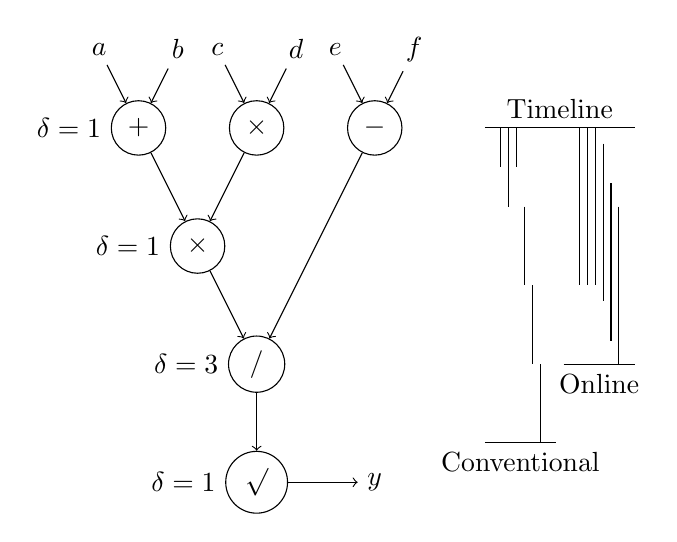
\begin{tikzpicture}
  \path
  (-0.5,5)   node(a) {$a$}
  (0.5,5)    node(b) {$b$}
  (1.0,5)    node(c) {$c$}
  (2,5)      node(d) {$d$}
  (2.5,5)    node(e) {$e$}
  (3.5,5)    node(f) {$f$}

  (0,4)      node[circle,draw,label=left:{$\delta=1$}](p1)  {$+$}
  (1.5,4)    node[circle,draw](p2)                          {$\times$}
  (3,4)      node[circle,draw](p3)                          {$-$}
  (0.75,2.5) node[circle,draw,label=left:{$\delta=1$}](p4)  {$\times$}
  (1.5,1)    node[circle,draw,label=left:{$\delta=3$}](p5)  {$/$}
  (1.5,-0.5) node[circle,draw,label=left:{$\delta=1$}](p6)  {$\surd$}

  (3,-0.5)   node(y) {$y$}
  ;

  \draw[->] (a) -- (p1);
  \draw[->] (b) -- (p1);
  \draw[->] (c) -- (p2);
  \draw[->] (d) -- (p2);
  \draw[->] (e) -- (p3);
  \draw[->] (f) -- (p3);

  \draw[->] (p1) -- (p4);
  \draw[->] (p2) -- (p4);
  \draw[->] (p3) -- (p5);
  \draw[->] (p4) -- (p5);
  \draw[->] (p5) -- (p6);

  \draw[->] (p6) -- (y);

  \draw (4.4,4) -- (6.3,4) node[midway,above]() {Timeline};;
  \draw (4.4,0) -- (5.3,0) node[midway,below]() {Conventional};
  \draw (5.4,1) -- (6.3,1) node[midway,below]() {Online};

  \draw (4.6,4) -- (4.6,3.5);
  \draw (4.7,4) -- (4.7,3);
  \draw (4.8,4) -- (4.8,3.5);
  \draw (4.9,3) -- (4.9,2);
  \draw (5.0,2) -- (5.0,1);
  \draw (5.1,1) -- (5.1,0);

  \draw (5.6,4) -- (5.6,2);
  \draw (5.7,4) -- (5.7,2);
  \draw (5.8,4) -- (5.8,2);
  \draw (5.9,3.8) -- (5.9,1.8);
  \draw (6.0,3.3) -- (6.0,1.3);
  \draw (6.1,3) -- (6.1,1);

\end{tikzpicture}
  \caption{Computing $y=\sqrt{(a+b)cd/(e-f)}$ with serial online operators~\cite{Ercegovac1}}
  \label{Online}
\end{figure}

As illustrated in figure~\ref{Online}, while each individual operation may take longer than its conventional counterpart, online arithmetic can provide a speedup if the operators are chained in serial.
In addition to the tradeoff in time, individual online arithmetic operators also uses more memory.
To perform all computation from the MSD to the LSD, the use of a redundant number system is compulsory.
However, this redundancy also has its advantage in making the operators scalable.
The time required per digit can be made independent of the length of the operands~\cite{Trivedi1}.

A recently proposed architecture allows the precision of online arithmetic to be controlled at runtime~\cite{Zhao1}.
Traditionally, this runtime control was restricted due to the parallel adders present in the multipliers and dividers.
This architecture reuses a fixed-precision adder and stores residues in on-chip RAM.
As such, a single piece of hardware can be used to calculate to any precision, limited only by the size of the on-chip RAM.

The way online arithmetic alleviates the second problem of fixed precision falls out directly from its MSD-first nature.
Suppose the output of a conventional ripple adder is sampled before it has completed its operation.
In this case, the lower digits would have been completed, but the carry would not have reached the higher ones.
This means the error on the result would be significant, as the top bits were still undetermined~\cite{Shi1}.
However, if the output of a parallel online adder is sampled before its completion, the lower bits would be the undetermined ones.
This means the error of the operation would be small.
With overclocking, online arithmetic operators fail gracefully, losing their precision gradually from the lowest bits first.
Thus, it allows for a runtime tradeoff between precision and frequency~\cite{Shi2}.

% REVISIT JD: find better arguments for high radix on FPGA for these two paras
\subsection{High-radix Arithmetic}
Conventional designs of arithmetic operators use binary representations.
The additional concerns of high-radix operators did not provide justifiable improvements as clock speed of processors kept increasing.
In recent years, the clock speed increase effectively ended, and semiconductor dies shrunk to extremely small sizes.
This means the relative processing time available in a clock period increased.
This enabled and drove the desire for accomplishing more per clock cycle, and high-radix arithmetic is one of them.
It has been shown that, high-radix offers power saving and/or reasonable speedups to the arithmetic operations~\cite{Catanzaro1}\cite{Amin1}\cite{Chen1}.

However, the savings are not without trade-offs.
If the radix chosen is not a power of 2, then this trade-off can become unfavourable if the specification requires much I/O and little computation.
This is because overhead of radix conversion would be significant~\cite{Whyte1}.
It is also unwise to use high-radix representations when the numbers are unusually small, thus making the savings offered by the high-radices negligible~\cite{Catanzaro1}.
The radix also cannot be too high, as the time in a clock period is still limited, if there is too many logic gates for the signal to propagate through, it might become the critical path and slow down the overall design.

The construct of FPGAs might make high-radices more attractive than it is on ICs.
As FPGAs contain small fast carry-ripple adders, high-radix adders may be able to exploit them to obtain significant speedups~\cite{Kornerup1}.

\subsection{High-radix Online Arithmetic}
Using high-radix number representations for online arithmetic is a relatively novel concept.
While there has been some research with similar premises~\cite{Lynch1}\cite{Lynch2}, We take a more direct approach with this project by implementing custom operators made for high-radix online arithmetic on an FPGA.
This will provide empirical results on the method, and will hopefully reveal practical insights along the way.

Furthermore, benchmarking this exotic arithmetic system with popular FPGA applications such as neural networks would be interesting, as there is not much precedence for it.


\newpage
\begin{thebibliography}{1}
% Unused:
% M. D. Ercegovac and T. Lang. Digital Arithmetic

\bibitem{Ahmed1}
  I. Ahmed, S. Zhao, J. Meijers, O. Trescases and V. Betz,
  ``\textit{Automatic BRAM Testing for Robust Dynamic Voltage Scaling for
  FPGAs}'',
  \textit{Int. Conf. on Field-Programmable Logic and Applications},
  2018.

\bibitem{Amin1}
  A Amin, W. Shinwari,
  ``\textit{High-Radix Multiplier-Dividers: Theory, Design, and Hardware}'',
  \textit{IEEE Trans. Comput.}, vol. 1, no.8,
  2008.

\bibitem{Brent1}
  R.P. Brent,
  ``\textit{A Regular Layout for Parallel Adders}'',
  \textit{IEEE Trans. Comput.}, vol. C-31, pp. 260-264,
  1982.

\bibitem{Catanzaro1}
  B. Catanzaro, and B. Nelson,
  ``\textit{Higher Radix Floating-Point Representations for FPGA-Based
  Arithmetic}'',
  \textit{Proceedings of the 51st Annual Design Automation Conference},
  2005.

\bibitem{Chen1}
  L. Chen, F. Lombardi, P. Montuschi, J. Han and W. Liu,
  ``\textit{Design of Approximate High-Radix Dividers by Inexact Binary
  Signed-Digit Addition}'',
  \textit{Proceedings of the on Great Lakes Symposium on VLSI},
  2017.

\bibitem{Duncan1}
  R. Duncan,
  ``\textit{A Survey of Parallel Computer Architectures}'',
  \textit{Computer}, vol. 23, pp. 5-16,
  1990.

\bibitem{Duran1}
  J.W. Duran,
  ``\textit{An Evaluation of Random Testing}'',
  \textit{IEEE Trans. on Software Engineering}, vol. SE-10, no. 4, pp. 438-444,
  1984.

\bibitem{Ercegovac1}
  M.D. Ercegovac,
  ``\textit{On-line Arithmetic: An Overview}'',
  \textit{28th Annual Technical Symposium}, pp. 86-93,
  Internaltional Society for Optics and Photonics,
  1984.

\bibitem{Ercegovac2}
  M.D. Ercegovac, and T. Lang,
  ``\textit{Digital Arithmetic}'',
  Morgan Kaufmann,
  2003.

\bibitem{Hazwani1}
  S. Hazwani, et al,
  ``\textit{Randomness Analysis of Pseudo Random Noise Generator Using 24-bits
  LFSR}'',
  \textit{Fifth Int. Conf. on Intelligent Systems, Modelling and Simulation},
  2014.

\bibitem{Kornerup1}
  P. Kornerup,
  ``\textit{Reviewing High-Radix Signed-Digit Adders}'',
  \textit{IEEE Trans. Comput.}, vol.64, no. 5, pp. 1502-1505,
  2015.

\bibitem{Li1}
  H. Li, J.J. Davis, J. Wickerson and G.A. Constantinides,
  ``\textit{ARCHITECT: Arbitrary-precision Constant-hardware Iterative
  Compute}'',
  \textit{Int. Conf. on Field-Programmable Technology},
  2017.

\bibitem{Lynch1}
  T. Lynch, and M.J. Schulte,
  ``\textit{A High Radix On-line Arithmetic for Credible and Accurate
  Computing}'',
  \textit{Journal of Universal Computer Science}, vol. 1, no. 7, pp. 439-453,
  1995.

\bibitem{Lynch2}
  T. Lynch, and M.J. Schulte,
  ``\textit{Software for High Radix On-line Arithmetic}'',
  \textit{Reliable Computing}, vol. 2, no. 2, pp. 133-138,
  1996.

\bibitem{Marsaglia1}
  G. Marsaglia,
  ``\textit{Xorshift RNGs}'',
  \textit{Journal of Statistical Software},
  2003.

\bibitem{Srinivas1}
  H.R. Srinivas, and K.K. Parhi,
  ``\textit{High-Speed VLSI Arithmetic Processor Architectures Using Hybrid
  Number Representation}'',
  \textit{J. of VLSI Sign. Process.}, vol. 4. pp. 177-198,
  1992.

\bibitem{Shi1}
  K. Shi, D. Boland, and G.A. Constantinides,
  ``\textit{Accuracy-Performance Tradeoffs on an FPGA through Overclocking}'',
  \textit{Proc. Int. Symp. Field-Programmable Custom Computing Machines},
  pp. 29-36,
  2013.

\bibitem{Shi2}
  K. Shi, D. Boland, E. Stott, S. Bayliss, and G.A. Constantinides,
  ``\textit{Datapath Synthesis for Overclocking: Online Arithmetic for
  Latency-Accuracy Trade-offs}'',
  \textit{Proceedings of the 13th Symposium on Field-Programmable Custom
  Computing Machines},
  pp. 1-6, ACM,
  2014.

\bibitem{Scekic1}
  O. Šćekić
  ``\textit{FPGA Comparative Analysis}'',
  \textit{University of Belgrade},
  2005.

\bibitem{Tenca1}
  A.F. Tenca, and M.D. Ercegovac,
  ``\textit{Design of high-radix digit-slices for on-line computations}'',
  2007.

\bibitem{Trivedi1}
  K.S. Trivedi, and M.D. Ercegovac,
  ``\textit{On-line Algorithms for Division and Multiplication}'',
  \textit{IEEE Trans. Comput.}, vol. C-26, no. 7, pp. 667-680,
  1977.

\bibitem{Whyte1}
  P. Whyte,
  ``\textit{Design and Implementation of High-radix Arithmetic Systems Based
  on the SDNR/RNS Data Representation}''
  \textit{Edith Cowan University},
  1997.

\bibitem{Zhao1}
  Y. Zhao, J. Wickerson, and G.A. Constantinides,
  ``\textit{An Efficient Implementation of Online Arithmetic}'',
  \textit{Int. Conf. on Field-Programmable Technology},
  2016.

% ------------------------------------------------------------------------------

\bibitem{Accellera1}
  Accellera Systems Initiative,
  ``\textit{Universal Verification Methodology 1.2 User’s Guide}'',
  2015.
  % Available at:\\\url{https://accellera.org/images/downloads/standards/uvm/
  % uvm_users_guide_1.2.pdf}.

\bibitem{Altera1}
  Altera Corporation,
  ``\textit{Cyclone V SoC Development Board Reference Manual}'',
  2015.
  % Available at:\\\url{www.intel.com/content/dam/www/programmable/us/en/pdfs/
  % literature/manual/rm_cv_soc_dev_board.pdf}.

\bibitem{Altera2}
  Altera Corporation,
  ``\textit{Memory System Design}'',
  \textit{Embedded Design Handbook},
  2010.
  % Available at:\\\url{www.intel.com/content/dam/www/programmable/us/en/pdfs/
  % literature/hb/nios2/edh_ed51008.pdf}.

\bibitem{Altera3}
  Altera Corporation,
  ``\textit{Introduction to Altmemphy IP}'',
  \textit{External Memory Interface Handbook: Reference Material}, vol. 3,
  2012.
  % Available at:\\\url{www.intel.com/content/dam/www/programmable/us/en/pdfs/
  % literature/hb/external-memory/emi_ddr3_ug.pdf}

\bibitem{Altera4}
  Altera Corporation,
  ``\textit{Phase-Locked Loop Basics, PLL}''.
  % Available at:\\\url{https://www.intel.com/content/www/us/en/programmable/
  % support/support-resources/operation-and-testing/pll-and-clock-management/
  % pll-basics.html}

\bibitem{Altera5}
  Altera Corporation,
  ``\textit{Creating Qsys Components}'',
  2018.
  % Available at:\\\url{https://www.intel.com/content/dam/www/programmable/us/
  % en/pdfs/literature/hb/qts/qsys_components.pdf}.

\bibitem{Altera6}
  Altera Corporation,
  ``\textit{Cyclone V Hard Processor System Technical Reference Manual}'',
  2018.
  % Available at:\\\url{https://www.intel.com/content/dam/www/programmable/us/
  % en/pdfs/literature/hb/cyclone-v/cv_54005.pdf}.

\bibitem{Altera7}
  Altera Corporation,
  ``\textit{Implementing Fractional PLL Reconfiguration with Altera PLL and
  Altera PLL Reconfig IP Cores}''.
  % Available at:\\\url{https://www.intel.com/content/dam/www/programmable/us/
  % en/pdfs/literature/an/an661.pdf}

\bibitem{Imperial1}
  Imperial College
  ``\textit{An Ethics Code}'',
  \textit{Imperial College Research Ethics Committee},
  2013.

\bibitem{Intel1}
  Intel Corporation,
  ``\textit{Cyclone V SoC Development Kit and Intel SoC FPGA Embedded
  Development Suite}''.
  % Available at:\\\url{www.intel.com/content/www/us/en/programmable/products/
  % boards_and_kits/dev-kits/altera/kit-cyclone-v-soc.html}.

\bibitem{Intel2}
  Intel Corporation,
  ``\textit{Introduction to Intel FPGA IP Cores}'',
  2018.
  % Available at:\\\url{https://www.intel.com/content/www/us/en/programmable/
  % documentation/mwh1409960636914.html}.

\bibitem{Intel3}
  Intel Corporation,
  ``\textit{Avalon Interface Specifications}'',
  2018.
  % Available at:\\\url{https://www.intel.com/content/dam/www/programmable/us/
  % en/pdfs/literature/manual/mnl_avalon_spec.pdf}.

\bibitem{Intel4}
  Intel Corporation,
  ``\textit{Cyclone V Device Overview}'',
  2018.
  % Available at:\\\url{https://www.intel.com/content/dam/www/programmable/us/
  % en/pdfs/literature/hb/cyclone-v/cv_51001.pdf

\bibitem{Rocket1}
  RocketBoards.org,
  ``\textit{GSRD 14.1 User manual}'',
  2015.
  % Available at:\\\url{https://rocketboards.org/foswiki/Documentation/GSRD141}.

\bibitem{Xilinx1}
  Xilinx, Inc,
  ``\textit{Zynq-7000 All Programmable SoC}'',
  2018.
  % Available at:\\\url{www.xilinx.com/support/documentation/
  % product-briefs/zynq-7000-product-brief.pdf}.

\bibitem{Xilinx2}
  Xilinx, Inc,
  ``\textit{ZedBoard (Zynq Evaluation and Development) Hardware User's Guide}'',
  2012.
  % Available at:\\\url{https://reference.digilentinc.com/_media/
  % zedboard:zedboard_ug.pdf}.
\end{thebibliography}

\end{document}